\subsection{Annotation Schema}

The primary goal of annotation is to provide a reduced set of searchable,
understandable data that can hint at relationships between logged 
events and guide the user to further searches and to interesting locations
in the raw log data. Along with our identified requirements, this 
provides some design requirements for the schema:

\begin{figure}
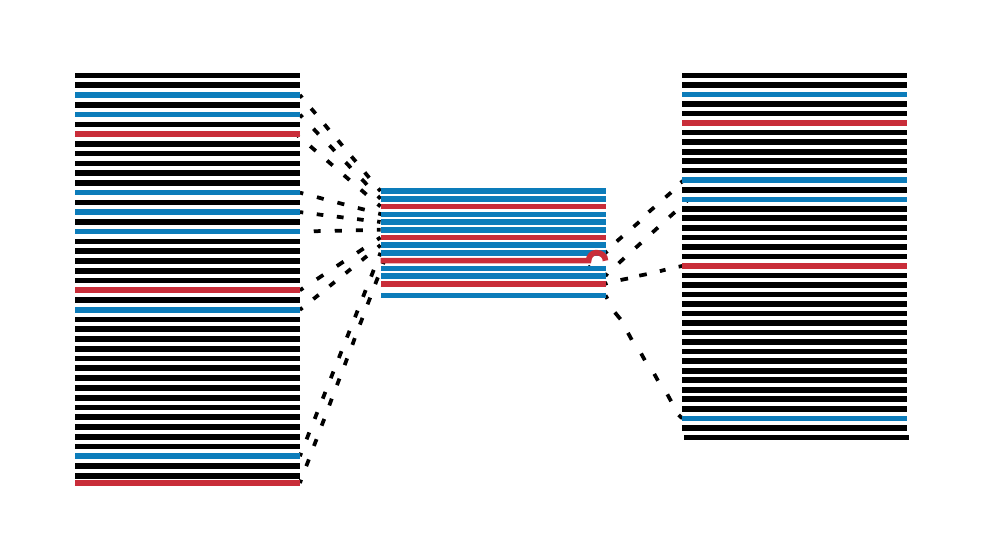
\includegraphics[width=0.4\textwidth]{annotations.png}
\caption{Annotations provide reduced, tractable view of significant events
in a much larger volume of log data.}
\label{f:annotations}
\end{figure}

\begin{itemize}
\item Temporal and subject (system and component) information are 
      the key fields, along with a human readable description, the 
      annotation itself.
\item The raw logfiles that the annotation concerns should be identified,
      if possible.
\item Multiple people should be able to annotate the same underlying 
      log data, and users of the annotations should be able to 
      identify annotators to request more information, if necessary.  
\item The architectural relationships between components indicated in 
      annotations should be accessible, in order to facilitate 
      traversal from an annotation of interest to annotations relating to
      components that may have impacted it.
\item Annotation fields should support searching based on the subject type 
      of an annotated event (such as a network event) or other 
      related information.
\end{itemize}

\subsubsection{The schema}

%In this subsection we describe the major fields necessary to support the
%architectural requirements that pertain to the annotations themselves
%(as opposed to the remote discovery infrastructure). The prototype
%implementation is an SQLite database, so we descirbe in in terms
%of that implemention, however that is not required. More generally
%this would be descirbed in terms of accessor APIs independent of
%the implementation beneath them.
Our annotation schema can be represented as an SQL database definition with a central 
``annotations'' table:

\begin{figure}[H]
\begin{small}
\begin{minted}{sql}
CREATE TABLE 'annotations' (
       id             integer,
       authorid       char(3) NOT NULL,
       description    text NOT NULL,
       -- timespan of the action or event:
       starttime      datetime NOT NULL,
       endtime        datetime NOT NULL,
       -- impact of the action or event:
       startstate     text,
       endstate       text,
       systemdown     boolean,
       system         text,
       components     text,
       -- was the event manually induced?
       manual         boolean,
       -- subject type and annotation context:
       LDcategory     text,
       LDtag          text,
       balerpatternid integer,
       -- event source:
       logfiles       text,
       PRIMARY KEY('id','authorid')
        );
\end{minted}
\end{small}
\caption{The central annotations table definition. }
\label{f:ann-table}
\end{figure}

The id, source, description and temporal fields are self-explanatory. 
The impact fields are designed to aid exploratory analysis, for example
\texttt{startstate} and \texttt{endstate} can be used to indicate that
a component that was in a \texttt{faulty} was either \texttt{repaired}
or \texttt{flagged} by the end of the event. A \texttt{systemdown} flag
allows search for events resulting in a full system failure.

The \texttt{system} and \texttt{components} fields correspond to the 
\texttt{Subject} class of the RDF vocabulary.
For the Cray system we define \texttt{node}, \texttt{blade}, \texttt{chassis},
\texttt{cabinet}, \texttt{router}, \texttt{tile}, \texttt{link}, \texttt{nic},
\texttt{smw}, and \texttt{other}, all of which (except \texttt{other}) are 
also \texttt{SubjectType}s described in RDF in data dictionaries and can, in
combination with the \texttt{system}, identify a specific component.

The \texttt{components} may be identified with finer granularity than
is represented in the RDF graph - for example \texttt{c0-1c0s4n0}. The 
\texttt{LDcategory} includes \texttt{node/blade},
\texttt{scheduler}, \texttt{storage}, \texttt{network}, 
\texttt{cooling/facilities/sensors},
\texttt{power}, \texttt{system software}, \texttt{datawarp}, 
and \texttt{unknown}, which also correspond (except for \texttt{unknown}) to
 \texttt{SubjectType}s in an RDF dictionary. The name of this field and its 
 categories are inspired by LogDiver~\cite{LogDiver}, 
a tool developed by UIUC which associates regular expressions defining
events in log files of interest with categorizations including these. 
We envisage LogDiver as an option used to identify log entries for annotation.

The \texttt{manual} flag indicates that an event was manually induced,
such as an administrator action to take down a node as opposed
to the system taking down a node because it failed a health check.
Knowledge of this can be used to more accurately determine the
number of true failure events and for assessing the effectiveness
and availability of system resilience mechanisms


% not sure ofthe context here... (other tables?):
%Note that event may have many relationships. We choose to limit them to one each to address
%the requirement of searchability. It is expected that exploration will facilitate dsicovery
%of events, even when the first order assocation may be off; also discovery of assocationed
%events in different subsytems can help understanding of how events propagate in a system.


\subsubsection{Other tables}

The schema includes some supporting tables:

\begin{description}
\item[Meta Annotations] \hfill

      The \texttt{metaannotations} table supports annotation sets,
      wherein a collection of annotations relates to a single larger
      event
      
\item[Component Aliases] \hfill

      Different components are identified differently in different log 
      series, for example the same node on a Cray XC might be called
      \texttt{nid00001} by the scheduling system, \texttt{c0-0c0s0n1}
      by the boot system and even its IP address by another log source.
      
      To support this we define an \texttt{aliases} table, mapping 
      equivalent component names. This is generally populated via
      \texttt{/etc/hosts}, or on Cray systems, the output from
      \texttt{rtr --system-map}
      
\item[Architectures] \hfill

      The topologies of current clusters are more complex than
      a simple hierarchy, so we support the definition of multiple
      architectures to describe relationships between components.
      We have defined three architectures for Cray systems, these
      are described below. 
      %in Section~\ref{s:hierarchies}.
      We chose to separate architectures in order to enable different
search and interpretation of events which affect components with
different \texttt{association} with each other. 
\texttt{associations}
include \texttt{parent-child: component-component} as opposed to
\texttt{parent-child: router-tile}, or \texttt{peer: HSN link}
as opposed to \texttt{peer: Router-NIC} or \texttt{peer: NIC-Proc}.

      
\end{description}

\subsubsection{Component hierarchies}
\label{s:hierarchies}

We have identified three distinct architectures within a Cray cluster

\begin{enumerate}
\item The \texttt{physical} architecture consists of parent-child or
container-contained associations, such as a \texttt{cabinet - chassis}, 
\texttt{blade - router}, \texttt{router - link} and \texttt{router - nic}.
This table is populated from the system definition - for example on a 
Cray XC each cabinet holds three chassis, so an entry might look like:

\begin{small}
\begin{verbatim}
id  type  cname  parent  children
1   CAB   c0-0   smw     c0-0c0,c0-0c1,c0-0c2
\end{verbatim}
\end{small}

The \texttt{physical} architecture supports discovery of faults 
propagating from child to parent components and vice versa.

\item The \texttt{router} architecture describes network topology
from the perspective of the router - for example an Aries may be specified by its 
(blue:black:green) identifiers  while a Gemini by its X:Y:Z. This 
supports determination of proximity of events in the network topology.

\begin{small}
\begin{verbatim}
id  type  cname        NICS [...]   nettopo
10  RTR   c0-0c0s10a0  c0-0cd0...   0:0:10
11  RTR   c0-0c0s11a0  c0-0c0s...   0:0:11
12  RTR   c0-0c1s0a0   c0-0c1s...   0:1:0
13  RTR   c0-0c1s1a0   c0-0c1s...   0:1:1
\end{verbatim}
\end{small}

\item The \texttt{link} architecture supports 
discovery of faults propagating across connected components,
such as a node failure disabling a link and contributing to 
congestion conditions on its peer node.

\begin{small}
\begin{verbatim}
id  type E0            E1            
16  GRE  c0-0c0s0a0l20 c0-0c0s4a0l22 
\end{verbatim}
\end{small}

\end{enumerate}

A few components, such as the SMW affect everything in the system. To represent 
such global associations we also define
a \texttt{supremum} relationship.



%In the prototype, we define all architectures and relationships,
%however we currently prinipally search the physical topology only
%and support recursive search up and down, including for supremum
%relationships. We are working on tools to better enable search of
%the multiple architecture represenations.
%
%In order to determine the effect of events on jobs, we also
%intend that job data be made availble with the annotations.
%We expect only the current common fields (e.g., starttime,
%endtime, components, etc) exposed in scheulder logs or
%interfaces.







